\section{Gate model of computation}
%%%%%%%%%%%%%%%%%%%%%%%%%%%%%%%%%%%%%%%%%%%%%%%%%%%%%%%%%%%%%%%%%%%%%%%%%%%%%%%%
\begingroup
\nologo
\begin{frame}{Gate model}
\begin{block}{How to perform computations?}
\begin{itemize}
\item Prepare the system in a known state, eg.: $\ket{0} \otimes \ket{1}$.
\item Apply quantum gates and partial measurements on the state.
\item Perform the measurement.
\item Analyze the result and post-processing. 
\end{itemize}
\end{block}
\vspace{0.5cm}
\begin{block}{Example of a quantum circuit}
\begin{figure}
\centering
\mbox{
\Qcircuit @C=1em @R=.7em { 
\lstick{\ket{0}} & \qw & \gate{H}  & \qw & \multigate{1}{U_f} & \qw 
& \gate{H} & \qw & \meter & \cw 
\\ 
\lstick{\ket{1}} & \qw & \gate{H} & \qw & \ghost{U_f} & \qw 
& \qw & \qw & \qw &  \qw 
}
}
\end{figure}
\end{block}
\end{frame}
\endgroup%%%%%%%%%%%%%%%%%%%%%%%%%%%%%%%%%%%%%%%%%%%%%%%%%%%%%%%%%%%%%%%%%%%%%%%%%%%%%%%%
\subsection{Classical gates}
%%%%%%%%%%%%%%%%%%%%%%%%%%%%%%%%%%%%%%%%%%%%%%%%%%%%%%%%%%%%%%%%%%%%%%%%%%%%%%%%
\begin{frame}{Classical gates}
\begin{columns}
\begin{column}[c]{0.5\textwidth}
\begin{circuitikz}[]
% something does not work here!
\node[buffer port] (BUF) at (0,0){};
\draw (BUF.out) -- ++(0.6,0) node[near end,above](Out){$x$};
\draw (BUF.in) -- ++(-0.2,0)node[left](In){$x$};
\end{circuitikz}\\[1cm]
\begin{circuitikz}[]
\node[not port] (NOT) at (0,0){};
\draw (NOT.out) -- ++(0.6,0) node[near end,above](Out){$\neg 
x$};
\draw (NOT.in) -- ++(-0.2,0)node[left](In){$x$};
\end{circuitikz}
\end{column}
\begin{column}[c]{0.5\textwidth}
\begin{circuitikz}[]
\node[or port] (OR) at (0,0){};
\draw (OR.out) -- ++(0.6,0) node[near end,above](Out){$x \text{ 
OR } y$};
\draw (OR.in 1) -- ++(-0.2,0)node[left](In1){$x$};
\draw (OR.in 2) -- ++(-0.2,0)node[left](In2){$y$};
\end{circuitikz}\\[1cm]
\begin{circuitikz}[]
\node[and port] (AND) at (0,0){};
\draw (AND.out) -- ++(0.6,0) node[near end,above](Out){$x 
\text{ AND } y$};
\draw (AND.in 1) -- ++(-0.2,0)node[left](In1){$x$};
\draw (AND.in 2) -- ++(-0.2,0)node[left](In2){$y$};
\end{circuitikz}\\[1cm]
\begin{circuitikz}[]
\node[xor port] (XOR) at (0,0){};
\draw (XOR.out) -- ++(0.6,0) node[near end,above](Out){$x 
\oplus y$};
\draw (XOR.in 1) -- ++(-0.2,0)node[left](In1){$x$};
\draw (XOR.in 2) -- ++(-0.2,0)node[left](In2){$y$};
\end{circuitikz}
\end{column}
\end{columns}
\end{frame}
%%%%%%%%%%%%%%%%%%%%%%%%%%%%%%%%%%%%%%%%%%%%%%%%%%%%%%%%%%%%%%%%%%%%%%%%%%%%%%%%
\subsection{Single qubit gates}
%%%%%%%%%%%%%%%%%%%%%%%%%%%%%%%%%%%%%%%%%%%%%%%%%%%%%%%%%%%%%%%%%%%%%%%%%%%%%%%%
\begin{frame}{Single qubit gate - unitary gate}
\begin{block}{How to denote a quantum single-qubit gate?}
\vspace{0.5cm}
\centering

\begin{tabular}{c c c}
$\ket{\psi}$ &
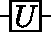
\includegraphics[valign=m, scale=1]{pics/unitary} &   $U \ket\psi$
\end{tabular}
\end{block}

\vspace{1cm}
\begin{block}{Quantum evolution is time-reversible!}
\begin{equation*}
U\ket{\psi_{t=0}} = \ket{\psi_{t=1}}
\end{equation*}
\begin{equation*}
U^\dagger\ket{\psi_{t=1}} = \ket{\psi_{t=0}}
\end{equation*}
\end{block}
\end{frame}
%%%%%%%%%%%%%%%%%%%%%%%%%%%%%%%%%%%%%%%%%%%%%%%%%%%%%%%%%%%%%%%%%%%%%%%%%%%%%%%%
\begin{frame}{Rotations}
\begin{columns}
\begin{column}[t]{0.35\textwidth}
\begin{center}
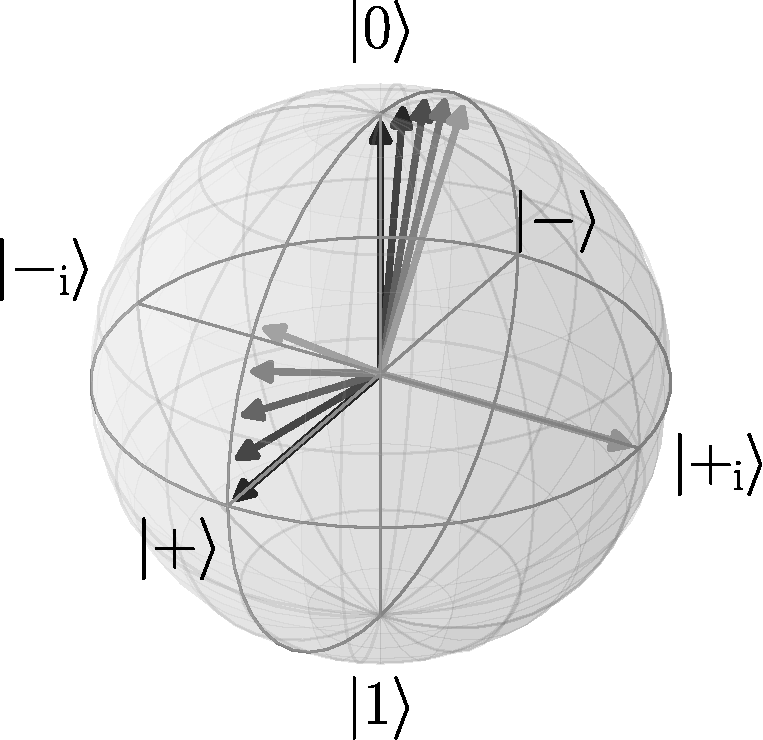
\includegraphics[width=0.9\textwidth]{pics/Ry} \\
$$
R_y(\gamma) = 
\begin{bmatrix}
\cos\left(\frac{\gamma}{2}\right) & \sin\left(\frac{\gamma}{2}\right)         \\
-\sin\left(\frac{\gamma}{2}\right) & \cos\left(\frac{\gamma}{2}\right)
\end{bmatrix}
$$
\end{center}
\end{column}
% \vrule{}
\begin{column}[t]{0.35\textwidth}
\begin{center}
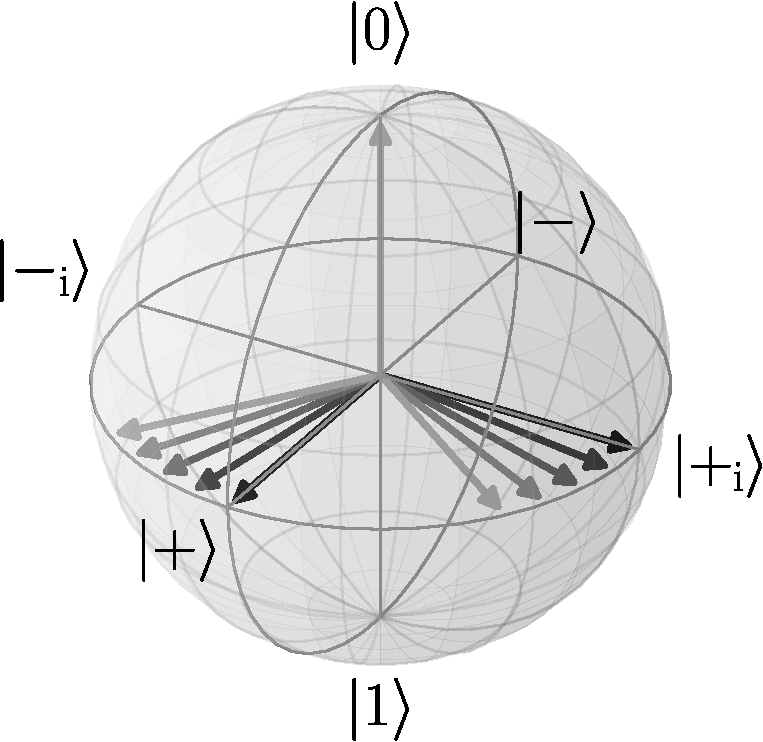
\includegraphics[width=0.9\textwidth]{pics/Rz} \\
$$
R_z(\beta) = 
\begin{bmatrix}
\mathrm{e}^{\frac{\mathrm{i} \beta}{2}} & 0        \\
0 & - \mathrm{e}^{\frac{\mathrm{i} \beta}{2}}
\end{bmatrix}
$$
\end{center}
\end{column}
\end{columns}
\end{frame}
%%%%%%%%%%%%%%%%%%%%%%%%%%%%%%%%%%%%%%%%%%%%%%%%%%%%%%%%%%%%%%%%%%%%%%%%%%%%%%%%
\begin{frame}{Important examples of single-qubit gates}
\centering
\begin{tabularx}{0.65\textwidth}{Xc}
\parbox[c]{\hsize}{
	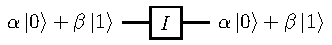
\includegraphics[page=1]{pics/single_qubit_gates.pdf}
} &
$
\begin{bmatrix}
1 & 0 \\
0 & 1
\end{bmatrix}
$
\\ [0.8cm]
\parbox[c]{\hsize}{
	\includegraphics[page=2]{pics/single_qubit_gates.pdf}
} &
$
\begin{bmatrix}
0 & 1 \\
1 & 0
\end{bmatrix}
$
\\[0.8cm]
\parbox[c]{\hsize}{
	\includegraphics[page=3]{pics/single_qubit_gates.pdf}
} &
$
\begin{bmatrix}
0 & -\mathrm{i}  \\
\mathrm{i} & 0
\end{bmatrix}
$
\\ [0.8cm]
\parbox[c]{\hsize}{
	\includegraphics[page=4]{pics/single_qubit_gates.pdf}
} &
$
\begin{bmatrix}
1 & 0         \\
0 & -1
\end{bmatrix}
$
\\ [0.8cm]
\parbox[c]{\hsize}{
	\includegraphics[page=5]{pics/single_qubit_gates.pdf}
} &
$
\begin{bmatrix}
1 & 0         \\
0 & \mathrm{e}^{\mathrm{i} \phi}
\end{bmatrix}
$
\end{tabularx}
\end{frame}

\begin{frame}{Hadamard gate}
\centering
$
H= \frac{1}{\sqrt{2}}\begin{bmatrix}
1 & 1         \\
1 & -1
\end{bmatrix},
$
\quad
$H\ket{0}=\frac{\ket{0}+\ket{1}}{\sqrt{2}}$, 
\quad
$H\ket{1}=\frac{\ket{0}-\ket{1}}{\sqrt{2}}$.
\\
\vspace{0.5cm}
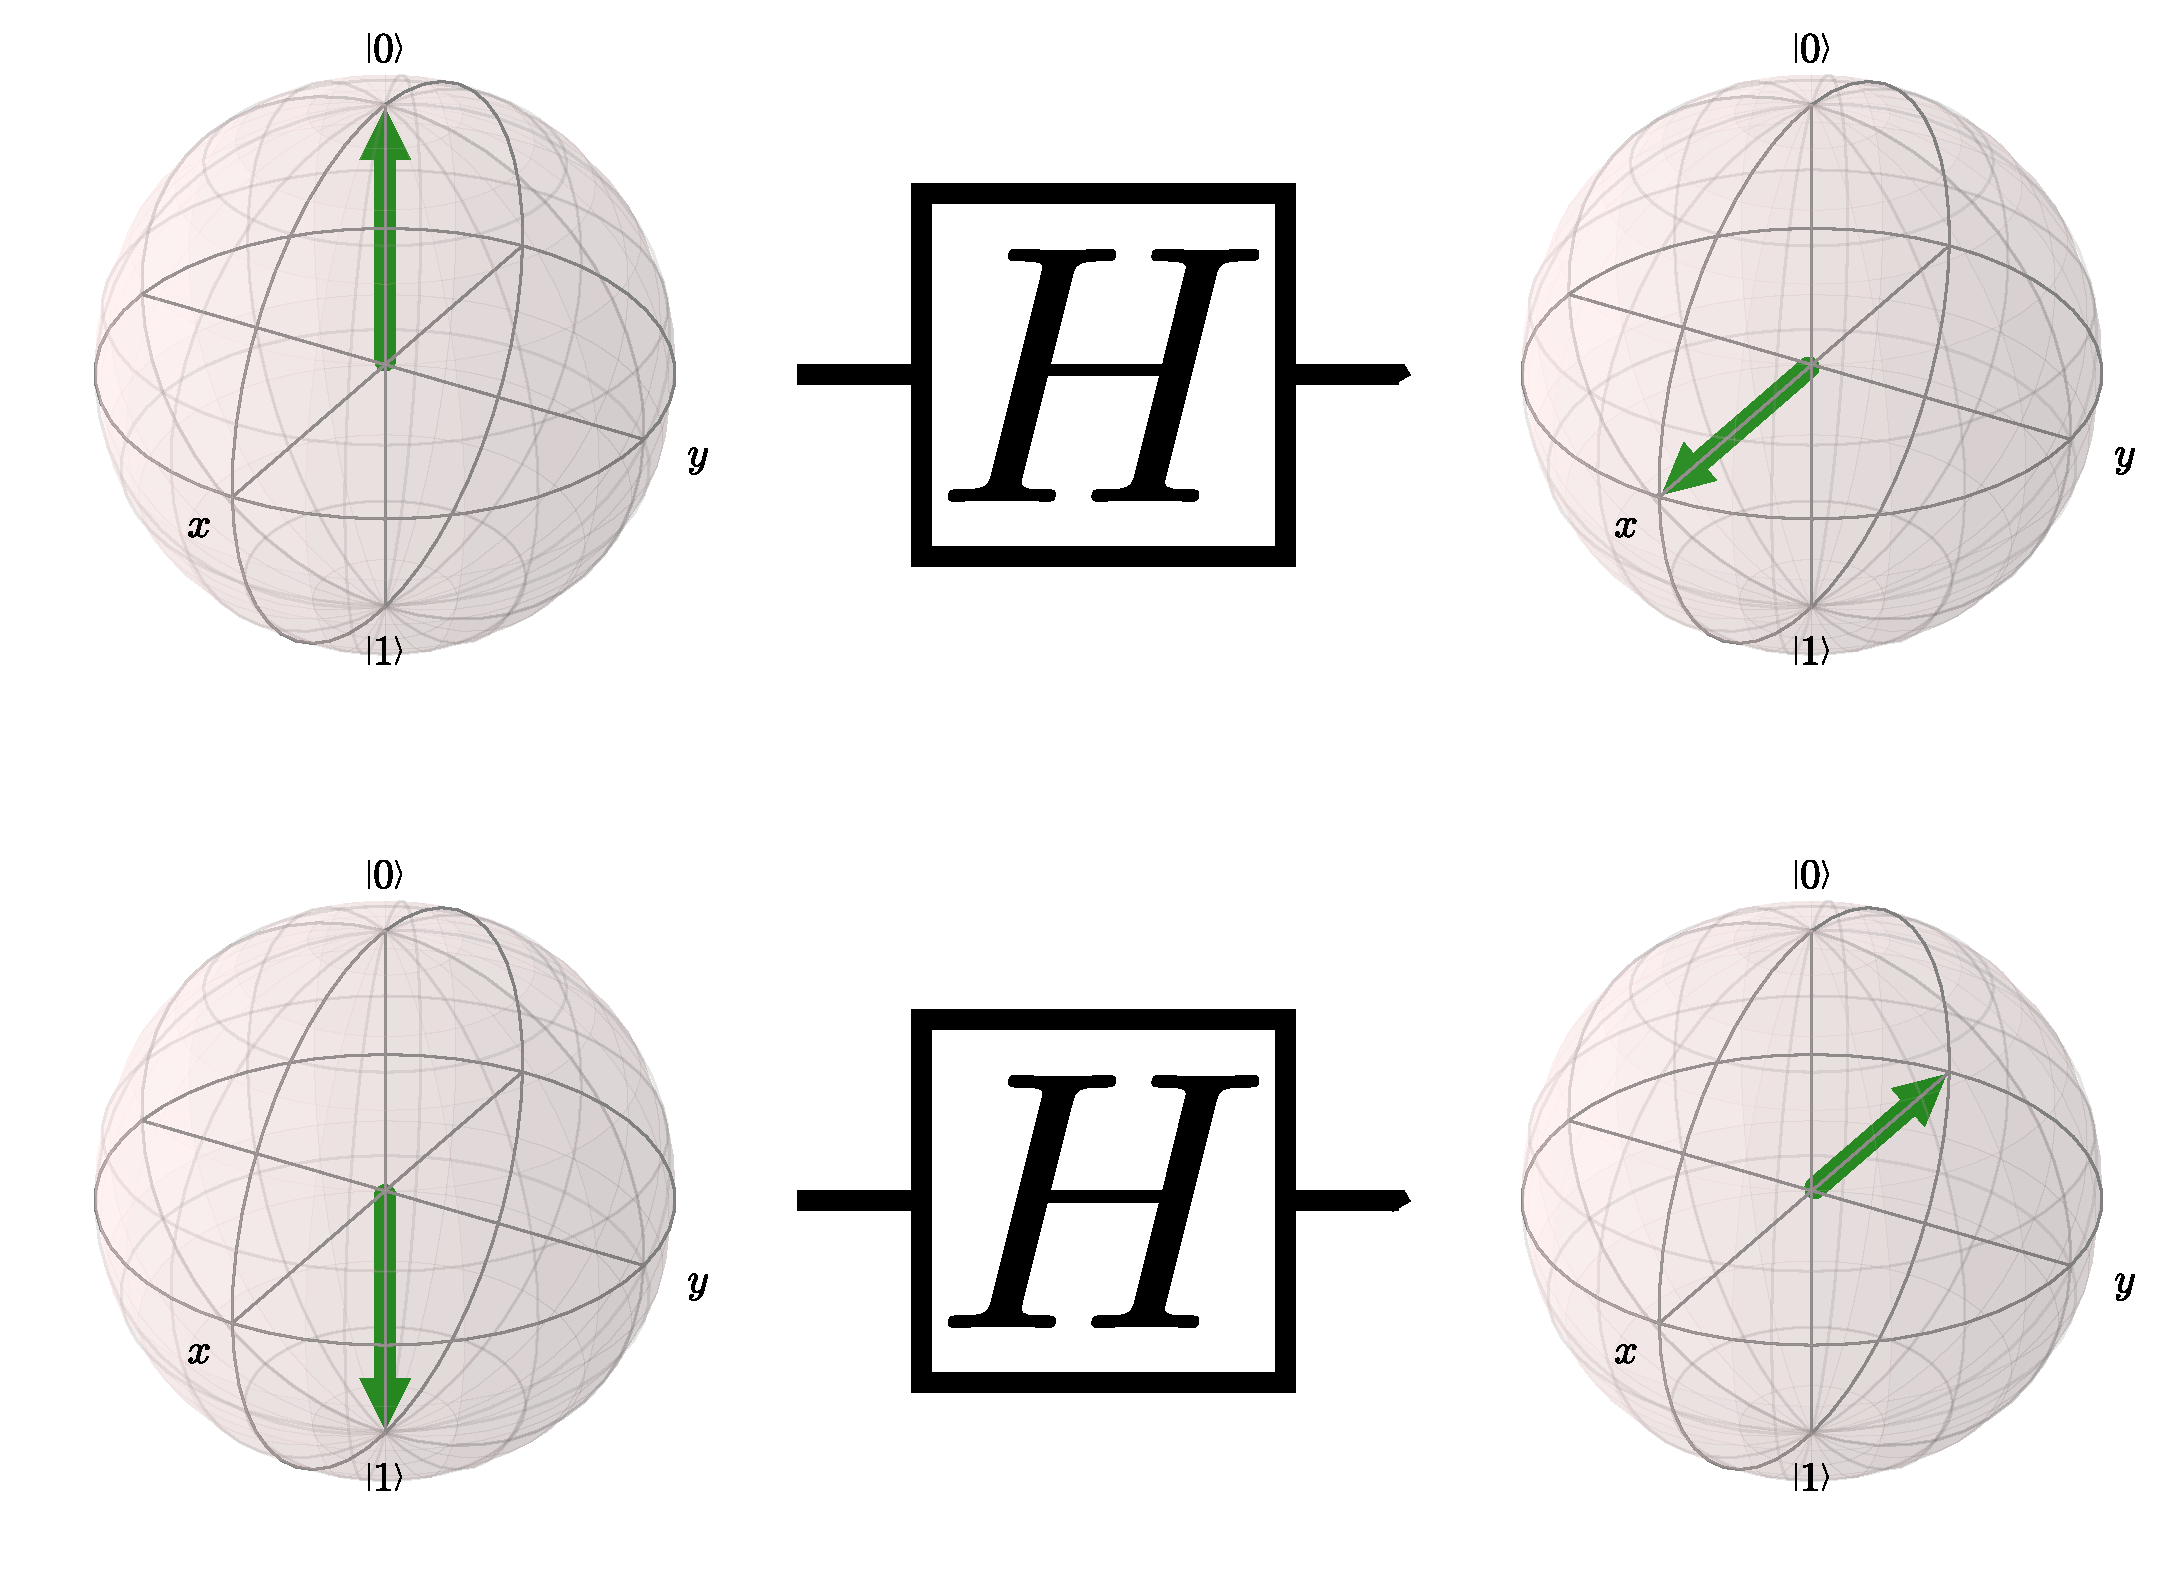
\includegraphics[width=0.5\textwidth]{pics/ewolucja}
\end{frame}

% % % % % % % % % % % % %

\begin{frame}{Decomposition of a unitary gate}
\begin{block}{Definition}
A square matrix is called \emph{unitary} iff 
\begin{equation*}
U U^\dagger = U^\dagger U = \mathbb{1}.
\end{equation*} 
\end{block}
\begin{block}{Every unitary gate $U$ can be written as}
\centering
%\begin{tabular}{c|c|c}
%UNITARY &
%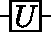
\includegraphics[valign=m, scale=1]{pics/unitary} &
%$U\ket{\psi_1} = \ket{\psi_2}$, $U^\dagger\ket{\psi_2} = \ket{\psi_1}$
%\end{tabular}
%\begin{figure}
%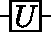
\includegraphics[valign=m, scale=1]{pics/unitary}
%\end{figure}

$$U = R_Z(\psi) R_Y (\theta) R_Z(\Delta)
=e^{i\varphi /2}{\begin{bmatrix}e^{i\psi }&0\\0&e^{-i\psi 
}\end{bmatrix}}{\begin{bmatrix}\cos \theta &\sin \theta \\-\sin \theta &\cos 
\theta \\\end{bmatrix}}{\begin{bmatrix}e^{i\Delta }&0\\0&e^{-i\Delta 
}\end{bmatrix}}.$$
\end{block}
\end{frame}

\begin{frame}{CNOT gate}
%\begin{block}{}
\centering
\begin{tabular}{c c}
%CNOT &
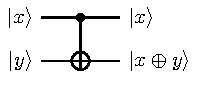
\includegraphics[valign=c,page=1,scale=1.1]{pics/two_qubit_gates.pdf} &
%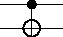
\includegraphics[valign=b, scale=2]{pics/cnot} &
\begin{tabular}{cc|cc}
$\text{in}_1$ & $\text{in}_2$ & $\text{out}_1$ & $\text{out}_2$ \\
\hline
0 & 0 & 0 & 0\\
0 & 1 & 0 & 1\\
1 & 0 & 1 & 1\\
1 & 1 & 1 & 0 
\end{tabular}
\end{tabular}
%\end{block}

\vspace{1.5cm}
\begin{tabularx}{\textwidth}{Xc}
\centering
%\parbox[c]{\hsize}{
%%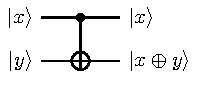
\includegraphics[page=1]{pics/two_qubit_gates.pdf}
%} &
$
\begin{bmatrix}
	1 & 0 & 0 & 0 \\
	0 & 1 & 0 & 0 \\
	0 & 0 & 0 & 1 \\
	0 & 0 & 1 & 0
\end{bmatrix}:
\begin{bmatrix}
	\alpha \\
	\beta  \\
	\gamma \\
	\delta
\end{bmatrix} \to
\begin{bmatrix}
	\alpha \\
	\beta  \\
	\delta \\
	\gamma
\end{bmatrix}
$
\end{tabularx}
\end{frame}

\begin{frame}{Controlled unitary}
%\begin{block}{}
\begin{tabularx}{0.8\textwidth}{Xc}

\parbox[c]{\hsize}{
\begin{figure}
\centering
\mbox{
\Qcircuit @C=2em @R=1em { 
 & \ctrl{1} & \qw \\ 
& \gate{U} & \qw }
}
\end{figure}
}
&
$
U=
\begin{bmatrix}
u_{00} & u_{01} \\
u_{10} & u_{11}
\end{bmatrix}
$
\end{tabularx}
%\end{block}
\vspace{0.8cm}

%\begin{block}{}
\begin{tabularx}{\textwidth}{Xc}
\centering
$
CU_1^2 =  \ketbra{0}{0} \otimes \mathbb{I} + 
\ketbra{1}{1} \otimes U = 
\begin{bmatrix}
	1 & 0 & 0 & 0 \\
	0 & 1 & 0 & 0 \\
	0 & 0 & u_{00} & u_{01} \\
	0 & 0 & u_{10} & u_{11}
\end{bmatrix}
$
\end{tabularx}
%\end{block}

\end{frame}


\subsection{2-qubit gates}
%%%%%%%%%%%%%%%%%%%%%%%%%%%%%%%%%%%%%%%%%%%%%%%%%%%%%%%%%%%%%%%%%%%%%%%%%%%%%%%%
\begin{frame}{Swap gate}
\centering
\begin{tabularx}{0.8\textwidth}{Xc}
%\parbox[c]{\hsize}{
%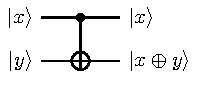
\includegraphics[page=1]{pics/two_qubit_gates.pdf}
%} &
%$
%\begin{bmatrix}
%	1 & 0 & 0 & 0 \\
%	0 & 1 & 0 & 0 \\
%	0 & 0 & 0 & 1 \\
%	0 & 0 & 1 & 0
%\end{bmatrix}:
%\begin{bmatrix}
%	\alpha \\
%	\beta  \\
%	\gamma \\
%	\delta
%\end{bmatrix} \to
%\begin{bmatrix}
%	\alpha \\
%	\beta  \\
%	\delta \\
%	\gamma
%\end{bmatrix}
%$   \\[0.8cm]
\parbox[c]{\hsize}{
\includegraphics[page=2]{pics/two_qubit_gates.pdf}
}
&
$
\begin{bmatrix}
	1 & 0 & 0 & 0 \\
	0 & 0 & 1 & 0 \\
	0 & 1 & 0 & 0 \\
	0 & 0 & 0 & 1
\end{bmatrix}:
\begin{bmatrix}
	\alpha \\
	\beta  \\
	\gamma \\
	\delta
\end{bmatrix} \to
\begin{bmatrix}
	\alpha \\
	\gamma \\
	\beta  \\
	\delta
\end{bmatrix}
$   \\[1.8cm]
\parbox[c]{\hsize}{
\includegraphics[page=3]{pics/two_qubit_gates.pdf}
}
&
$
\begin{bmatrix}
	1 & 0             & 0             & 0 \\
	0 & \frac{1+i}{2} & \frac{1-i}{2} & 0 \\
	0 & \frac{1-i}{2} & \frac{1+i}{2} & 0 \\
	0 & 0             & 0             & 1
\end{bmatrix}:
\begin{bmatrix}
	\alpha \\
	\beta  \\
	\gamma \\
	\delta
\end{bmatrix} \to
\begin{bmatrix}
	\alpha                                   \\
	\frac{1+i}{2}\beta + \frac{1-i}{2}\gamma \\
	\frac{1-i}{2}\beta + \frac{1+i}{2}\gamma \\
	\delta
\end{bmatrix}
$
\end{tabularx}
\end{frame}

\begin{frame}{Example of a circuit}
\begin{figure}
\centering
\mbox{
\Qcircuit @C=1em @R=.7em { 
\lstick{\ket{0}} & \qw & \gate{H}  & \qw &\ctrl{1} & \qw \\
\lstick{\ket{0}} & \qw & \qw  & \qw  & \targ & \qw
}
}
\end{figure}
%\centering
% 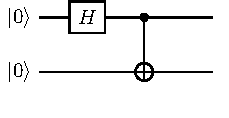
\includegraphics[page=1]{pics/example_of_quantum_circuit.pdf}
\begin{enumerate}
\item $(H \otimes I)\ket{0} \otimes \ket{0} =
\frac{1}{\sqrt{2}} \left( \ket{0} + \ket{1} \right) \otimes \ket{0}
= 
\frac{1}{\sqrt{2}}
\begin{bmatrix}
1 \\
0 \\
1 \\
0
\end{bmatrix}
$

\item
$ \begin{bmatrix}
	1 & 0 & 0 & 0 \\
	0 & 1 & 0 & 0 \\
	0 & 0 & 0 & 1 \\
	0 & 0 & 1 & 0
\end{bmatrix}
%\frac{1}{\sqrt{2}}
\begin{bmatrix}
\frac{1}{\sqrt{2}} \\
0 \\
\frac{1}{\sqrt{2}} \\
0
\end{bmatrix}
= 
\begin{bmatrix}
\frac{1}{\sqrt{2}} \\
0 \\
0 \\
\frac{1}{\sqrt{2}} 
\end{bmatrix}
= \frac{1}{\sqrt{2}} \left(  \ket{00} + \ket{11} \right)
$
\end{enumerate}
\end{frame}

\subsection{Deutsch algorithm}

\begin{frame}{Deutsch algorithm -- problem formulation}

\begin{itemize}
\item Consider a function $f:\{0,1\}^N \rightarrow\{0,1\}$ that is either constant or balanced (i.e. half of its values are $0$s and the other half are $1$s).
\item For $N=1$ each function is either constant or balanced.
\end{itemize}
\begin{table}
\begin{tabular}{c|c c c}
& $f(0)$ & $f(1)$ & \\
\hline
$f_0$ & $0$ & $0$ & \multirow{2}{*}{constant}\\
$f_1$ & $1$ & $1$ & \\
\hline
identity & $0$ & $1$ & \multirow{2}{*}{balanced}\\
bit flip & $1$ & $0$ & \\ 
\end{tabular}
\end{table}
\begin{block}{Problem}
Given $f$ decide if it is constant or balanced.
\end{block}
\end{frame}

\begin{frame}{Hadamard transform}
\begin{columns}
	\column[c]{0.4\textwidth}
	\begin{figure}
		\centering
		\mbox{
		\Qcircuit @C=1em @R=.7em { 
		\lstick{\ket{0}} & \qw & \gate{H} & \qw & \qw \\ 
		\lstick{\ket{0}} & \qw & \gate{H} & \qw & \qw \\
		&& \vdots &&  \\
		 \\
		\lstick{\ket{0}} & \qw & \gate{H} & \qw & \qw 
		}
		}
		\end{figure}
	\column{0.6\textwidth}
	Hadamard transform creates an equal superposition of all possible states of the system. 


	For two qubits we have:
	\begin{equation*}
	\begin{split}
	\left(H \otimes H \right)\ket{00}
	&= \left(  \frac{\ket{0} + \ket{1}}{\sqrt{2}} \right) \otimes
	\left(  \frac{\ket{0} + \ket{1}}{\sqrt{2}} \right) \\
	&= \frac{1}{2} \left( \ket{00} + \ket{01} + \ket{10} + 
	\ket{11}\right).
	\end{split}
	\end{equation*}
	
	And more generally:
	\begin{equation*}
	H^{\otimes N} \ket{0}^{\otimes N} = \frac{1}{\sqrt{2^N}} \sum_{x \in \{0, 1\}^N} \ket{x}.
	\end{equation*}
\end{columns}
\end{frame}

\begin{frame}{Black box}
\begin{columns}
\begin{column}{0.65\textwidth}
To implement Deutsch's algorithm we need \\
a black box computing the following:
\begin{equation*}
U_f\ket{x,y} = \ket{x, y \oplus f(x)} 
\end{equation*}
%Notice that $U_f$ is unitary.
\end{column}
\begin{column}{0.3\textwidth}
\begin{table}
\begin{tabular}{c c | c}
$x$ & $y$ & $y \oplus x$ \\
\hline
$0$ & $0$ & $0$ \\
$0$ & $1$ & $1$ \\
$1$ & $0$ & $1$ \\
$1$ & $1$ & $0$ 
\end{tabular}
\end{table}
\end{column}
\end{columns}
\vspace{0.5cm}
\begin{figure}
\centering
\mbox{
\Qcircuit @C=1em @R=.7em { 
& \ustick{x} \qw  & \qw  & \multigate{1}{U_f} & \qw& \ustick{x} \qw &   \qw & \qw  \\
& \dstick{y} \qw  & \qw  &  \ghost{U_f}        & \qw & \qw & \dstick{y \oplus f(x)}   \qw &  \qw 
}
}
\end{figure}
\end{frame}
% \beta 
\begin{frame}{Black box}
We can express $U_f$ in a way that will be useful later. For instance
\begin{equation*}
U_f\ket{00} = \ket{0, 0\oplus f(0)} = \begin{cases}
\ket{00} & \mbox{ if } f(0) = 0 \\
\ket{01} & \mbox{ if } f(0) = 1, 
\end{cases}
\end{equation*} 
and hence
\begin{equation*}
U_f\ket{00} = (1 - f(0))\ket{00} + f(0)\ket{01}.
\end{equation*}

Also
\begin{equation*}
\begin{split}
U_f\ket{01} &= f(0)\ket{00} + (1-f(0))\ket{01}, \\
U_f\ket{10} &= (1-f(1))\ket{10} + f(1)\ket{11}, \\
U_f\ket{11} &= f(1)\ket{10} + (1-f(1))\ket{11}. 
\end{split}
\end{equation*}
\end{frame}

\begin{frame}{Deutsch algorith}
\begin{block}{}
\begin{figure}
\centering
\mbox{
\Qcircuit @C=1em @R=.7em { 
\lstick{\ket{0}} & \qw & \gate{H}  & \qw & \multigate{1}{U_f} & \qw 
& \gate{H} & \qw & \meter & \cw 
\\ 
\lstick{\ket{1}} & \qw & \gate{H} & \qw & \ghost{U_f} & \qw 
& \qw & \qw & \qw &  \qw 
}
}
\end{figure}
\end{block}

\begin{block}{Algorithm}
\begin{enumerate}
\item Apply the Hadamard transform to the input state $\ket{01}$. 
%to produce a product state of two superpositions.
\item Apply $U_f$ to the product state.
\item Apply the Hadamard gate to the first qubit.
\item Measure the first qubit.
\end{enumerate}
\end{block}
\end{frame}
%%%%%%%%%%%%%%%%%%%%%%%%%%%%%%%%%%%%%%%%%%%%%%%%%%%%%%%%%%%%%%%%%%%%%%%%%%%%%%%%

%\begin{frame}{Deutsch algorithm - problem formulation}
%\begin{itemize}
%\item There is a function $f:\{0,1\}\rightarrow\{0,1\}$
%\item Is $f$ constant $f(0)=f(1)$, or balanced $f(0)=\neg f(1)$?
%\end{itemize}
%\centering
%\begin{columns}
%\begin{column}{0.48\textwidth}
%\begin{block}{Constant functions}
%\includegraphics[page=2]{pics/deutsch.pdf}\ \ \ \
%\includegraphics[page=3]{pics/deutsch.pdf}
%\end{block}
%\end{column}
%\begin{column}{0.48\textwidth}
%\begin{block}{Balanced functions}
%\includegraphics[page=4]{pics/deutsch.pdf}\ \ \ \
%\includegraphics[page=5]{pics/deutsch.pdf}
%\end{block}
%\end{column}
%\end{columns}
%\end{frame}

%\begin{frame}{Deutsch algorithm}
%% see PTI 2021
%\begin{center}
%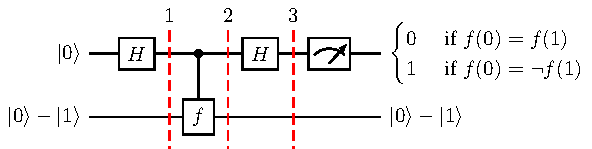
\includegraphics[page=1]{pics/deutsch.pdf}
%\end{center}
%\vspace{-0.5cm}
%\begin{enumerate}
%\item $\ket{0}+\ket{1}$
%\item  $(-1)^{f(0)}\ket{0}+(-1)^{f(1)}\ket{1} \equiv
% \ket{0}+(-1)^{f(0)}(-1)^{f(1)}\ket{1}
% = \ket{0}+(-1)^{f(0)\oplus f(1)}\ket{1}=$
%$=\begin{cases}
%  \ket{0}+\ket{1} & \text{for $f(0)\oplus f(1)=0$} \\
%  \ket{0}-\ket{1} & \text{for $f(0)\oplus f(1)=1$}
% \end{cases}
%$
%\item $\begin{cases}
%  \ket{0} & \text{for constant $f$}            \\
%  \ket{1} & \text{for injective $f$}
% \end{cases}
%$
%\end{enumerate}
%\end{frame}

\begin{frame}{Deutsch algorithm --- part I}
\begin{itemize}
\item Apply the Hadamard transform to the input state $\ket{01}$. 
\begin{equation*}
\begin{split}
\ket{\psi_1} &= \left(H \otimes H\right) \ket{01} = \left( \frac{\ket{0} + \ket{1}}{\sqrt{2}}\right) \otimes \left( \frac{\ket{0} - \ket{1}}{\sqrt{2}}\right) \\
& =\frac{1}{2} \left( \ket{00} - \ket{01}+ \ket{10} - \ket{11} \right)
\end{split}
\end{equation*}

\item Apply $U_f$ to the product state.
\begin{equation*}
\begin{split}
\ket{\psi_2} &= 
U_f \ket{\psi_1}
=   \frac{1}{2} \left( U_f\ket{00} - U_f \ket{01}+ U_f \ket{10} - U_f \ket{11} \right) \\
&= \frac{1-2f(0)}{2}  \ket{0} \otimes (\ket{0}- \ket{1})  
 + \frac{1-2f(1)}{2}  \ket{1} \otimes (\ket{0}- \ket{1})
\end{split}
\end{equation*}
\end{itemize}
\end{frame}


\begin{frame}{Deutsch algorithm --- part II}
\begin{itemize}
\item Apply the Hadamard gate to the first qubit.
\begin{equation*}
\begin{split}
\ket{\psi_3} =
(H \otimes I) \ket{\psi_2} 
&= \left( 1-f(0) -f(1) \right) \ket{0} \otimes
\frac{\ket{0}-\ket{1}}{\sqrt{2}} \\
&\quad  + \left( f(1) -f(0) \right) \ket{1} \otimes \frac{\ket{0}-\ket{1}}{\sqrt{2}}
\end{split}
\end{equation*}

\item Measure the first qubit.
\end{itemize}
\end{frame}

\begin{frame}{Deutsch-Jozsa algorithm}
\begin{block}{Question}
Is binary function $f:\{0,1\}^N\rightarrow\{0,1\}$ constant or balanced?
\end{block}
\vspace{1cm}
\begin{block}{Circuit for $N=2$}
\begin{figure}
\centering
\mbox{
\Qcircuit @C=1em @R=.7em { 
\lstick{\ket{0}} & \qw & \gate{H}  & \qw & \multigate{2}{U_f} & \qw 
& \gate{H} & \qw & \meter & \cw 
\\
\lstick{\ket{0}} & \qw & \gate{H}  & \qw & \ghost{U_f} & \qw 
& \gate{H} & \qw & \meter & \cw 
\\ 
\lstick{\ket{1}} & \qw & \gate{H} & \qw & \ghost{U_f} & \qw 
& \qw & \qw & \qw &  \qw 
}
}
\end{figure}
where $U_f\ket{x,x,y} = \ket{x,x, y \oplus f(x)} $.
\end{block}
\end{frame}

\begin{frame}{Deutsch-Jozsa algorithm}
\begin{figure}
\centering
\mbox{
\Qcircuit @C=1em @R=.7em { 
\lstick{\ket{0}^{\otimes N}} & \qw & \gate{H^{\otimes N}}  & \qw & \multigate{1}{U_f} & \qw 
& \gate{H^{\otimes N}} & \qw & \meter & \cw 
\\ 
\lstick{\ket{1} \quad} & \qw & \gate{H} & \qw & \ghost{U_f} & \qw 
& \qw & \qw & \qw &  \qw 
}reddreddredd
}
\end{figure}
\begin{block}{Algorithm}
\begin{enumerate}
\item Apply the Hadamard transform to the input state 
$\ket{0} \otimes \cdots \otimes \ket{0} \otimes \ket{1}$. 
%to produce a product state of two superpositions.
\item Apply $U_f$ to the product state, where
\begin{equation*}
U_f\ket{x, \ldots, x,y} = \ket{x,\ldots,x, y \oplus f(x)}. 
\end{equation*}
\item Apply the Hadamard gate to the first $N$ qubits.
\item Measure the first $N$ qubits.
\end{enumerate}
\end{block}
\end{frame}

\subsection{Teleportation}
\begin{frame}{Teleportation --- vision}
    \centering
    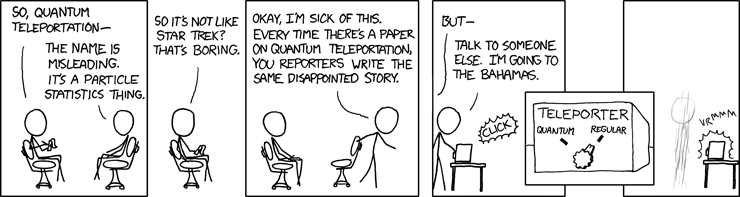
\includegraphics[width=\textwidth]{pics/teleportation/quantum_teleportation}\\
    {\footnotesize Source: \texttt{http://xkcd.com/465/} \copyright Randall Munroe 2015, CC-BY/2.5.}
\end{frame}

\begin{frame}{Teleportation --- theory}
    \centering
    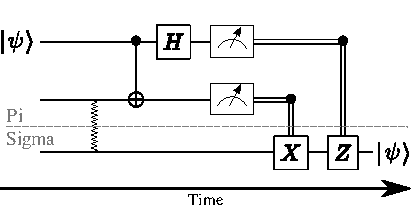
\includegraphics[width=\textwidth]{pics/teleportation/teleportation}
\end{frame}


\begin{frame}{Teleportation --- theory}
    \centering
    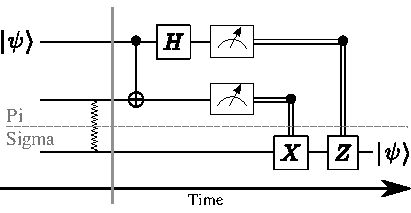
\includegraphics[width=0.45\textwidth]{pics/teleportation/teleportation_t0}
	\begin{equation*}
		\begin{split}
		\ket{\psi_{t=0}} &=  \ket{\psi} \otimes \ket{\Phi^+}  =\\
%			&= \ket{\psi} \otimes \frac{1}{\sqrt{2}}\left( \ket{0} \otimes \ket{0} +\ket{1} \otimes \ket{1} \right) = \\
			&= \left(\alpha \ket{0} + \beta  \ket{1}\right) \otimes \frac{1}{\sqrt{2}}\left( \ket{0} \otimes \ket{0} +\ket{1} \otimes \ket{1} \right)= \\
			&= \frac{1}{\sqrt{2}} \left(\alpha \ket{000} + \alpha \ket{011} + \beta  \ket{100} + \beta  \ket{111}  \right)
		\end{split}
	\end{equation*}
\end{frame}

\begin{frame}{Teleportation --- theory}
	\centering
    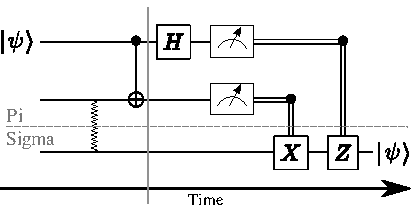
\includegraphics[width=0.45\textwidth]{pics/teleportation/teleportation_t1}
	\begin{equation*}
		\begin{split}
			\ket{\psi_{t=1}} &= (\mat{CNOT}_1^2\otimes \mathbb{I}) \frac{1}{\sqrt{2}} \left(\alpha \ket{000} + \alpha \ket{011} + \beta \ket{100} + \beta \ket{111}  \right) =\\
			&=\frac{1}{\sqrt{2}} \left(\alpha \ket{000} + \alpha \ket{011} + \beta \ket{110} + \beta \ket{101}  \right).
		\end{split}
	\end{equation*}
\end{frame}

\begin{frame}{Teleportation --- theory}
    \centering
	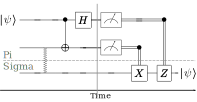
\includegraphics[width=0.45\textwidth]{pics/teleportation/teleportation_t2}
	\begin{equation*}
		\begin{split}
			\ket{\psi_{t=2}} &=( \mat{H}\otimes\mathbb{I}\otimes\mathbb{I}) \frac{1}{\sqrt{2}} \left(\alpha \ket{000} + \alpha \ket{011} + \beta \ket{110} + \beta \ket{101}  \right) =\\
			&= \frac{1}{\sqrt{2}} \Big(
			\alpha \frac{1}{\sqrt{2}}(\ket{0}+\ket{1})\otimes (\ket{00} +  \ket{11}) + \beta \frac{1}{\sqrt{2}}(\ket{0}-\ket{1})\otimes(\ket{10} + \ket{01}) \Big) =\\
			&= \frac{1}{2} \alpha(\ket{000} + \ket{100}  + \ket{011} + \ket{111}) + \frac{1}{2}\beta (\ket{010} + \ket{001} - \ket{110} - \ket{101})
		\end{split}
	\end{equation*}
\end{frame}

\begin{frame}{Teleportation --- theory}
    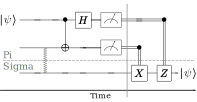
\includegraphics[width=0.45\textwidth]{pics/teleportation/teleportation_t3}
    \centering
\begin{equation*}
\begin{split}
\mathcal{P} = \{&\mat{P}_{00?}=\ketbra{0}{0}\otimes\ketbra{0}{0}\otimes\mathbb{I}, \mat{P}_{01?}=\ketbra{0}{0}\otimes\ketbra{1}{1}\otimes\mathbb{I}, \\
&\mat{P}_{10?}=\ketbra{1}{1}\otimes\ketbra{0}{0}\otimes\mathbb{I}, \mat{P}_{11?}=\ketbra{1}{1}\otimes\ketbra{1}{1}\otimes\mathbb{I}\}
\end{split}
\end{equation*}
\begin{itemize}
	\item result $00?$: $\frac{1}{\sqrt{2}}\left(\alpha \ket{000}  + \beta \ket{001}\right) = \frac{1}{\sqrt{2}}\left(\ket{00}\otimes \ket{\psi}\right)$,
	\item result $01?$: $\frac{1}{\sqrt{2}}\left(\alpha \ket{011}  + \beta \ket{010}\right) = \frac{1}{\sqrt{2}}\left(\ket{01}\otimes \mat{Z}\ket{\psi}\right)$,
	\item result $10?$: $\frac{1}{\sqrt{2}}\left(\alpha \ket{100}  - \beta \ket{101}\right) = \frac{1}{\sqrt{2}}\left(\ket{10}\otimes \mat{X}\ket{\psi}\right)$,
	\item result $11?$: $\frac{1}{\sqrt{2}}\left(\alpha \ket{111}  - \beta \ket{110}\right) = \frac{1}{\sqrt{2}}\left(\ket{11}\otimes \mat{X}\mat{Z}\ket{\psi}\right)$
\end{itemize}
\end{frame}

% \begin{frame}{Teleportation --- practice}
%     \centering
% 	\begin{block}{Architecture}
% 		\centering
% 	    \includegraphics[width=0.4\textwidth]{pics/IBM_architecture}  
% 	\end{block}

% 	\begin{block}{Circuit\footnote{\texttt{https://quantumexperience.ng.bluemix.net/qstage/\#/user/herrier}}}
% 		\centering
% 	    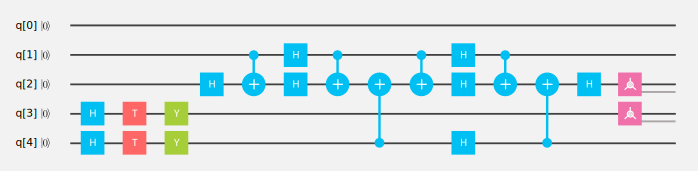
\includegraphics[width=\textwidth]{pics/teleportation_circuit}
% 	\end{block}
% \end{frame}

% \begin{frame}{Teleportation --- practice}
%     \centering
% 	\begin{block}{Results}
% 		\centering
% 	    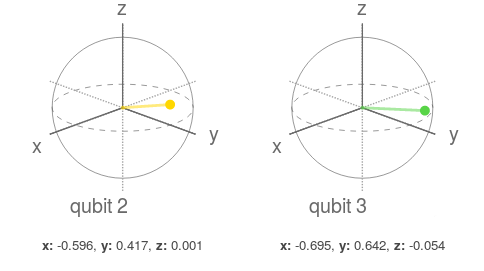
\includegraphics[width=0.9\textwidth]{pics/teleportation_blochs}  
% 	\end{block}
% \end{frame}

% \begin{frame}[fragile]{Teleportation --- practice}
% \begin{block}{QASM 2.0}
% \begin{columns}
% \begin{column}{0.30\textwidth}
% \begin{verbatim}
% include "qelib1.inc";
% qreg q[5];
% creg c[5];

% h q[3];
% h q[4];
% t q[3];
% t q[4];
% y q[3];
% \end{verbatim}
% \end{column}
% \begin{column}{0.30\textwidth}
% \begin{verbatim}
% y q[4];
% h q[2];
% cx q[1],q[2];
% h q[1];
% h q[2];
% cx q[1],q[2];
% cx q[4],q[2];
% cx q[1],q[2];
% h q[1];
% \end{verbatim}
% \end{column}
% \begin{column}{0.30\textwidth}
% \begin{verbatim}
% h q[2];
% h q[4];
% cx q[1],q[2];
% cx q[4],q[2];
% h q[2];
% bloch q[2];
% bloch q[3];
% \end{verbatim}
% \end{column}

% \end{columns}

% \end{block}
% \end{frame}